%%% The main file. It contains definitions of basic parameters and includes all other parts.

%% Settings for single-side (simplex) printing
% Margins: left 40mm, right 25mm, top and bottom 25mm
% (but beware, LaTeX adds 1in implicitly)
\documentclass[12pt,a4paper]{report}
\setlength\textwidth{145mm}
\setlength\textheight{247mm}
\setlength\oddsidemargin{15mm}
\setlength\evensidemargin{15mm}
\setlength\topmargin{0mm}
\setlength\headsep{0mm}
\setlength\headheight{0mm}
% \openright makes the following text appear on a right-hand page
\let\openright=\clearpage

%% Settings for two-sided (duplex) printing
% \documentclass[12pt,a4paper,twoside,openright]{report}
% \setlength\textwidth{145mm}
% \setlength\textheight{247mm}
% \setlength\oddsidemargin{14.2mm}
% \setlength\evensidemargin{0mm}
% \setlength\topmargin{0mm}
% \setlength\headsep{0mm}
% \setlength\headheight{0mm}
% \let\openright=\cleardoublepage

%% Generate PDF/A-2u
\usepackage[a-2u]{pdfx}

%% Character encoding: usually latin2, cp1250 or utf8:
\usepackage[utf8]{inputenc}

%% Prefer Latin Modern fonts
\usepackage{lmodern}

%% Further useful packages (included in most LaTeX distributions)
\usepackage{amsmath}        % extensions for typesetting of math
\usepackage{amsfonts}       % math fonts
\usepackage{amsthm}         % theorems, definitions, etc.
\usepackage{bbding}         % various symbols (squares, asterisks, scissors, ...)
\usepackage{bm}             % boldface symbols (\bm)
\usepackage{graphicx}       % embedding of pictures
\usepackage{fancyvrb}       % improved verbatim environment
\usepackage{natbib}         % citation style AUTHOR (YEAR), or AUTHOR [NUMBER]
\usepackage[nottoc]{tocbibind} % makes sure that bibliography and the lists
			    % of figures/tables are included in the table
			    % of contents
\usepackage{dcolumn}        % improved alignment of table columns
\usepackage{booktabs}       % improved horizontal lines in tables
\usepackage{paralist}       % improved enumerate and itemize
\usepackage[usenames]{xcolor}  % typesetting in color

%% my packages
\usepackage{algorithm}
\usepackage{algpseudocode}
\usepackage{mathtools}
\usepackage[acronym,toc]{glossaries}
\usepackage[toc,page,titletoc]{appendix}
% \usepackage{dirtree}

%%% Basic information on the thesis

% Thesis title in English (exactly as in the formal assignment)
\def\ThesisTitle{Automatic Point Clouds Merging}

% Author of the thesis
\def\ThesisAuthor{Jiří Hörner}

% Year when the thesis is submitted
\def\YearSubmitted{2018}

% Name of the department or institute, where the work was officially assigned
% (according to the Organizational Structure of MFF UK in English,
% or a full name of a department outside MFF)
\def\Department{Department of Theoretical Computer Science and Mathematical Logic}

% Is it a department (katedra), or an institute (ústav)?
\def\DeptType{Department}

% Thesis supervisor: name, surname and titles
\def\Supervisor{RNDr. David Obdržálek, Ph.D.}

% Supervisor's department (again according to Organizational structure of MFF)
\def\SupervisorsDepartment{Department of Theoretical Computer Science and Mathematical Logic}

% Study programme and specialization
\def\StudyProgramme{Computer Science}
\def\StudyBranch{Artificial Intelligence}

% An optional dedication: you can thank whomever you wish (your supervisor,
% consultant, a person who lent the software, etc.)
\def\Dedication{%
Dedication.
}

% Abstract (recommended length around 80-200 words; this is not a copy of your thesis assignment!)
\def\Abstract{%
Abstract.
}

% 3 to 5 keywords (recommended), each enclosed in curly braces
\def\Keywords{%
{key} {words}
}

%% The hyperref package for clickable links in PDF and also for storing
%% metadata to PDF (including the table of contents).
%% Most settings are pre-set by the pdfx package.
\hypersetup{unicode}
\hypersetup{breaklinks=true}

% create a glossary
\makeglossaries
% Definitions of acronyms
%%% Abbreviations used in the thesis, including their explanation

\newacronym{RANSAC}{RANSAC}{random sample consensus}
\newacronym{BFS}{BFS}{breadth-first search}
\newacronym{DFS}{DFS}{depth-first search}
\newacronym{ROS}{ROS}{Robot Operating System}
\newacronym{OpenCV}{OpenCV}{Open Source Computer Vision Library}
\newacronym{SIFT}{SIFT}{scale-invariant feature transform}
\newacronym{SLAM}{SLAM}{simultaneous localization and mapping}
\newacronym{FLANN}{FLANN}{Fast Library for Approximate Nearest Neighbors}
\newacronym{MIT}{MIT}{Massachusetts Institute of Technology}
\newacronym{GPS}{GPS}{Global Positioning System}
\newacronym{ICP}{ICP}{Iterative closest point}
\newacronym{AAU}{AAU}{Alpen-Adria-Universität Klagenfurt}
\newacronym{PFH}{PFH}{Point Feature Histogram}
\newacronym{PFHRGB}{PFHRGB}{Point Feature Histogram with colour}
\newacronym{FPFH}{FPFH}{Fast Point Feature Histogram}
\newacronym{SHOT}{SHOT}{Signature of Histograms of Orientations}
\newacronym{RSD}{RSD}{Radius-based Surface Descriptor}
\newacronym{SC3D}{SC3D}{3D Shape Context}
\newacronym{SAC-IA}{SAC-IA}{Sample Consensus Initial Alignment}
\newacronym{SVD}{SVD}{Singular-value decomposition}
\newacronym{API}{API}{Application Programming Interface}
\newacronym{PCL}{PCL}{Point Cloud Library}
\newacronym{NARF}{NARF}{Normal Aligned Radial Feature}


% Definitions of macros (see description inside)
%%% This file contains definitions of various useful macros and environments %%%
%%% Please add more macros here instead of cluttering other files with them. %%%

%%% Minor tweaks of style

% These macros employ a little dirty trick to convince LaTeX to typeset
% chapter headings sanely, without lots of empty space above them.
% Feel free to ignore.
\makeatletter
\def\@makechapterhead#1{
  {\parindent \z@ \raggedright \normalfont
   \Huge\bfseries \thechapter. #1
   \par\nobreak
   \vskip 20\p@
}}
\def\@makeschapterhead#1{
  {\parindent \z@ \raggedright \normalfont
   \Huge\bfseries #1
   \par\nobreak
   \vskip 20\p@
}}
\makeatother

% This macro defines a chapter, which is not numbered, but is included
% in the table of contents.
\def\chapwithtoc#1{
\chapter*{#1}
\addcontentsline{toc}{chapter}{#1}
}

% Draw black "slugs" whenever a line overflows, so that we can spot it easily.
\overfullrule=1mm

%%% Macros for definitions, theorems, claims, examples, ... (requires amsthm package)

\theoremstyle{plain}
\newtheorem{thm}{Theorem}
\newtheorem{lemma}[thm]{Lemma}
\newtheorem{claim}[thm]{Claim}

\theoremstyle{plain}
\newtheorem{defn}{Definition}

\theoremstyle{remark}
\newtheorem*{cor}{Corollary}
\newtheorem*{rem}{Remark}
\newtheorem*{example}{Example}

%%% An environment for proofs

%%% FIXME %%% \newenvironment{proof}{
%%% FIXME %%%   \par\medskip\noindent
%%% FIXME %%%   \textit{Proof}.
%%% FIXME %%% }{
%%% FIXME %%% \newline
%%% FIXME %%% \rightline{$\square$}  % or \SquareCastShadowBottomRight from bbding package
%%% FIXME %%% }

%%% An environment for typesetting of program code and input/output
%%% of programs. (Requires the fancyvrb package -- fancy verbatim.)

\DefineVerbatimEnvironment{code}{Verbatim}{fontsize=\small, frame=single}

%%% The field of all real and natural numbers
\newcommand{\R}{\mathbb{R}}
\newcommand{\N}{\mathbb{N}}

%%% Useful operators for statistics and probability
\DeclareMathOperator{\pr}{\textsf{P}}
\DeclareMathOperator{\E}{\textsf{E}\,}
\DeclareMathOperator{\var}{\textrm{var}}
\DeclareMathOperator{\sd}{\textrm{sd}}

%%% Transposition of a vector/matrix
\newcommand{\T}[1]{#1^\top}

%%% Various math goodies
\newcommand{\goto}{\rightarrow}
\newcommand{\gotop}{\stackrel{P}{\longrightarrow}}
\newcommand{\maon}[1]{o(n^{#1})}
\newcommand{\abs}[1]{\left|{#1}\right|}
\newcommand{\dint}{\int_0^\tau\!\!\int_0^\tau}
\newcommand{\isqr}[1]{\frac{1}{\sqrt{#1}}}

%%% Various table goodies
\newcommand{\pulrad}[1]{\raisebox{1.5ex}[0pt]{#1}}
\newcommand{\mc}[1]{\multicolumn{1}{c}{#1}}

%%% My macros

\DeclareMathOperator{\rank}{rank}
\DeclareMathOperator{\sgn}{sgn}
\DeclareMathOperator{\trace}{trace}
\DeclareMathOperator{\conv}{conv}
%\DeclareMathOperator{\R}{\mathbb{R}}
\DeclareMathOperator{\bigO}{\mathcal{O}}
\DeclarePairedDelimiter{\ev}{\operatorname{E}[}{]}
\DeclarePairedDelimiter{\prob}{\operatorname{P}[}{]}
%\DeclarePairedDelimiter{\abs}{\lvert}{\rvert}
\DeclarePairedDelimiter{\ceil}{\lceil}{\rceil}
\DeclarePairedDelimiter{\floor}{\lfloor}{\rfloor}
\DeclarePairedDelimiter{\norm}{\lVert}{\rVert}
\DeclarePairedDelimiter{\scal}{\langle}{\rangle}

\renewcommand{\algorithmicrequire}{\textbf{Input:}}
\renewcommand{\algorithmicensure}{\textbf{Output:}}

% ROS node API formatting
\newcommand{\ROStopic}[3]{\begin{sloppypar} \noindent\texttt{#1} (#2) \end{sloppypar} \par \hangindent=15pt \hangafter=0 \noindent #3}
\newcommand{\ROSparam}[4]{\begin{sloppypar} \noindent\texttt{#1} (#3, default: \texttt{#2}) \end{sloppypar} \par \hangindent=15pt \hangafter=0 \noindent #4}
\newcommand{\ROStransform}[3]{\begin{sloppypar} \noindent\texttt{#1} $\rightarrow$ \texttt{#2} \end{sloppypar} \par \hangindent=15pt \hangafter=0 \noindent #3}

% allow hyphenation after underscore
\let\oldunderscore\_
\renewcommand{\_}{\oldunderscore\-}

\hyphenation{mer-ged}
\hyphenation{cost-map}
\hyphenation{data-set}
% \hyphenation{sen-sor_-msgs/-Point-Cloud2}
\hyphenation{PFH-RGB}

\graphicspath {{../img/plots/}}


% Title page and various mandatory informational pages
\begin{document}
%%% Title page of the thesis and other mandatory pages

%%% Title page of the thesis

\pagestyle{empty}
\hypersetup{pageanchor=false}
\begin{center}

\centerline{\mbox{
\includegraphics[width=166mm]{../img/logo-en.pdf}}}

\vspace{-8mm}
\vfill

{\bf\Large MASTER THESIS}

\vfill

{\LARGE\ThesisAuthor}

\vspace{15mm}

{\LARGE\bfseries\ThesisTitle}

\vfill

\Department

\vfill

\begin{tabular}{rl}

Supervisor of the master thesis: & \Supervisor \\
\noalign{\vspace{2mm}}
Study programme: & \StudyProgramme \\
\noalign{\vspace{2mm}}
Study branch: & \StudyBranch \\
\end{tabular}

\vfill

% Zde doplňte rok
Prague \YearSubmitted

\end{center}

\newpage

%%% Here should be a bound sheet included -- a signed copy of the "master
%%% thesis assignment". This assignment is NOT a part of the electronic
%%% version of the thesis. DO NOT SCAN.

%%% A page with a solemn declaration to the master thesis

\openright
\hypersetup{pageanchor=true}
\pagestyle{plain}
\pagenumbering{roman}
\vglue 0pt plus 1fill

\noindent
I declare that I carried out this master thesis independently, and only with the cited
sources, literature and other professional sources.

\medskip\noindent
I understand that my work relates to the rights and obligations under the Act No.~121/2000 Sb.,
the Copyright Act, as amended, in particular the fact that the Charles
University has the right to conclude a license agreement on the use of this
work as a school work pursuant to Section 60 subsection 1 of the Copyright Act.

\vspace{10mm}

\hbox{\hbox to 0.5\hsize{%
In ........ date ............	% FIXME!
\hss}\hbox to 0.5\hsize{%
signature of the author
\hss}}

\vspace{20mm}
\newpage

%%% Dedication

\openright

\noindent
\Dedication

\newpage

%%% Mandatory information page of the thesis

\openright

\vbox to 0.5\vsize{
\setlength\parindent{0mm}
\setlength\parskip{5mm}

Title:
\ThesisTitle

Author:
\ThesisAuthor

\DeptType:
\Department

Supervisor:
\Supervisor, \SupervisorsDepartment

Abstract:
\Abstract

Keywords:
\Keywords

\vss}

\newpage

\openright
\pagestyle{plain}
\pagenumbering{arabic}
\setcounter{page}{1}


%%% A page with automatically generated table of contents of the master thesis

\tableofcontents

%%% Each chapter is kept in a separate file
\chapter*{Introduction}
\addcontentsline{toc}{chapter}{Introduction}

Multirobot systems are established research area within robotics and artificial intelligence with growing number of applications. The multirobot system can improve effectiveness both in the term of the performance and robustness over a single robot. A team of robots can also solve tasks that can not be tackled by the single robot. Multirobot systems can scale to large environments and the most demanding applications.

Multirobot systems have been deployed to several application domains including space exploration~\citep{goldberg2002distributedspace,huntsberger2003campout}, autonomous patrolling~\citep{parker2003parolling100}, disaster rescue and victim search, aerial surveillance, unmanned delivery, mine cleaning, snow removal~\citep{choset2001coverage}, assembly of large-scale buildings or planetary habitat~\citep{goldberg2002distributedspace} and robotic football~\citep{asada1999robocup}. Those applications require robots to operate in  dynamic environments, with high degree of uncertainty and external changes causes by other robots, humans and other agents that are not part of the multirobot system itself.

To be able to solve such demanding problems multirobot systems rely on distributed planning, communication, and control algorithms. This work presents an algorithm for estimating positions of the robots in the shared environment without any previous knowledge or assumptions about environment and for building the global map of the environment. Knowledge of positions of the robots and the map of the environment are crucial elements for effective collaborative planning and coordination. \textit{Unaware systems}~\citet{farinelli2004multirobot} that don't have knowledge of the presence of other robots are normally used only for very
simple tasks~\citet{farinelli2004multirobot}.

A typical multirobot system consists of many software parts typically structured in a multi-layer architecture. The implementation presented in this work leverages modularity of the widely-used \gls{ROS} framework and respects community established standards. This allows easy integration with existing planning, mapping and communication algorithms enabling quick development of multirobot systems suited for the particular task.

Chapter~\ref{chap:analysis} discusses related works and possible approaches to estimate robot positions in unknown environment. Chapter~\ref{chap:mergingalgorithm} introduces the implemented map-merging algorithm. Chapter~\ref{chap:implementation} presents implementation of the developed map-merging algorithm for the \gls{ROS} framework. Chapter~\ref{chap:evaluation} accesses performance of the implementation using several standard robotic datasets and experiments done by the author. Documentation for the \gls{ROS} implementation is attached as appendix~\ref{chap:map_merge-wiki}.

\chapter{Analysis}
\label{chap:analysis}

Knowledge of the positions of robots and knowledge of the environment is essential for solving complex tasks efficiently in multirobot systems. Over time various techniques evolved to acquire this knowledge.

\section{Map-merging}

This work focuses on multirobot systems consisting of mobile robots, each capable of building a \gls{3D} map of the surrounding environment. Typically each robot uses a \gls{SLAM} algorithm to create a map and is equipped with appropriate sensors such as stereo camera rigs, active \gls{RGB-D} cameras or laser range finders. Such sensors are available in the broad weight and cost range enabling large variety of \gls{SLAM}-capable robots operating both on the ground and in the air. This variety leads to possible heterogeneous teams of robots capable of solving broad range of tasks.

The \textit{map-merging problem} for multirobot systems, which is the focus of this work, is to estimate positions of the robots in the environment and to merge the maps from individual robots to produce a single globally consistent map.

\section{The map representation}

\Gls{3D} maps are becoming more common in the robotics as the capable sensors are getting more affordable and suitable for many applications. Unlike \gls{2D} occupancy grids used extensively in the past, \gls{3D} maps enable cooperation of robots, that are not fixed to a \gls{2D} plane, such as aerial vehicles, humanoid robots, outdoor robots operating in a rough terrain as well as traditional ground-based platforms. This allows us to create a possibly heterogeneous multirobot teams, that are able to take advantage of their different strengths and weaknesses to solve the assigned task efficiently. For example a robotic team can consist from aerial vehicles, capable of fast reconnaissance in large-scale outdoor environments, and ground-based vehicles carrying heavy equipment.

This work expects maps represented as pointclouds (definition~\ref{def:pointcloud}). Pointclouds can be implemented as an array of points, making them suitable for serialisation and exchange between robots. Points in the pointcloud can have assigned additional information, such as \gls{RGB} colour information or reflection intensity, based on the available sensor. Especially colour information, that is provided by stereo camera rigs and active \gls{RGB-D} cameras is commonly exploited for further processing.

\begin{defn}[Pointcloud]
\label{def:pointcloud}
A pointcloud is a set of data points in space.
\end{defn}

Other datastructures used in the \gls{3D} mapping, such as octree-based maps used by~\citet{hornung2013octomap}, can be converted to pointclouds without any loss of information, because pointclouds do not pose any restrictions on the geometry of the points and it is easy to add metadata associated with the points. This makes pointclouds suitable datastructure for exchange between different mapping approaches, even when they use different representations internally.

Pointclouds data messages are supported and well established in the \gls{ROS} framework. There are mature libraries to work with pointclouds, such as \gls{PCL}. This makes pointclouds suitable map representation for multi-robot systems.

\section{Direct map-merging}

Early map-merging techniques can be classified as \textit{direct map-merging}~\citet{lee2012survey}, which use direct sensor measurements to compute the transformation between robots. This involves especially the case of robot rendezvous~\citet{zhou2006rendezvous}, which relies on robots' ability to sense each other position directly. Popular technique uses camera and special recognizable markers on the robots to compute the transformation using computer vision algorithms.

A robot rendezvous might be hard to achieve in large-scale environments, especially if the robots are starting from different locations or in a different time (for example to react to increasing demands for a service). Such applications typically need map-merging to be able to work only with sensed surrounding environment instead of the presence of other robots in the same space.

Direct map-merging also involves techniques relying on global localization in the environment being available. This involves a purpose-adapted environments with installed markers or beacons to locate robots within environment and systems using global localization such as \gls{GPS}.

While purpose-adapted environments may greatly simplify map-merging problem, they make deployment of the multirobot systems harder and might introduce severe costs. For applications such as space exploration, disaster rescue, victim search and mine cleaning any modifications of the environment are not conceivable and in many more applications such as unmanned delivery the modifications are usually not practical.

Global localization systems are usually not available indoor and while such systems are a great aid for navigating large-scale outdoor environments, the provided accuracy is usually not high enough for merging high resolution pointcloud maps. The position from global localization system can be however used as an initial guess for map-merging algorithms.

\section{Map-merging on occupancy grids}

Later developed techniques work with \gls{2D} maps, usually represented as occupancy grids. \citet{lee2012survey}~categorizes this techniques as \textit{indirect map-merging}. These techniques rely on overlapping areas in maps for map-merging.

Using \gls{2D} maps limits operational space of robots and practically limits multirobot teams to only ground-based vehicles operating indoor or in light terrain flat environments. Particularly \gls{2D} maps prohibits promising multirobot teams consisting of aerial and ground-based vehicles.

Map-merging techniques on occupancy grinds involves spectra-based approach of~\citet{carpin2008spectra} and image feature-based approach of~\citet{Horner2016}. The latter algorithm is available in the \gls{ROS} distribution as ready-made solution for merging \gls{2D} maps.

\section{Map-merging as distributed SLAM}

Map-merging algorithms has been also implemented as distributed \gls{SLAM} algorithms. These techniques takes advantage of the research in the area of \gls{SLAM} algorithms and use loop-closure techniques developed for \gls{SLAM} to implement map-merging. Especially graph-based \gls{SLAM} implementations can be naturally extended to merge maps from multiple robots, nodes from other robots can be added to the graph and connected through the loop-closures with the existing nodes to form a single map.

When a loop-closure between 2 maps is detected, it can be used to compute the transformation between maps. We need to extend the loop detection to work across map boundaries, not only within a single map as usual in the \gls{SLAM}, which typically requires exchanging implementation-specific data between robots. This poses several disadvantages. Based on the \gls{SLAM} loop-closure approach the internal \gls{SLAM} data may be quite large, stressing communication bandwidth. Exchanging implementation-specific data usually leads to running the same \gls{SLAM} algorithm on all robots in the multirobot system, or the implementations must be adapted to exchange compatible loop-closure data. This is challenging for heterogeneous multirobot systems, when individual robots use different sensors, which is often the case when using both ground-based and aerial robots. For example if ground-based robots are equipped with accurate heavy \gls{3D} laser scanner and aerial vehicles use lightweight stereo rig cameras, the \gls{SLAM} approaches are typically different and the loop-closure data are incompatible (image features and \gls{3D} laser scans). In such scenarios we need to use different approach.

\citet{lee2012survey}~lists scan matching loop closures approaches used for map-merging, which are used with \gls{2D} \gls{SLAM} algorithms. \gls{2D} distributed \gls{SLAM} based on scan matching was implemented by~\citet{pfingsthorn2007scalable} for RoboCup Rescue Virtual Robots competition. \citet{fox2006distributed} used a direct exchange of laser range scans and odometry motion information coupled with a particle filter to localize robot in the second map.

In \gls{3D} camera-based \gls{SLAM} algorithms, visual appearance-based techniques are particularly popular. \citet{tomono2013merging} used appearance-based algorithm based on \gls{SIFT} features to merge visual maps, validated by travelled paths to reject false similarities in repetitive environments. Visual bag-of-words loop closure approach was used by~\citet{labbe2014online} to merge maps in multi-session \gls{SLAM}. Multi-session \gls{SLAM} works with maps generated by a single robot starting consecutively in the different positions. In such setup there is no need for communication, so a local database was used by the authors to store loop-closure related data for map-merging.

\section{Map-merging on pointclouds}

The algorithm presented in chapter~\ref{chap:mergingalgorithm} works exclusively with \gls{3D} pointclouds without any additional exchange of data to offer maximum flexibility. The algorithm does not require any exchange of implementation-specific data and can be used with any \gls{SLAM} approach available, allowing future integration of the newest state-of-the-art methods in face-paced \gls{SLAM} research. When the presented approach, each robot in the heterogeneous multirobot system can use different \gls{SLAM} implementation, which is best suited to its sensors and computational capabilities.

Using pointclouds can also save communication bandwidth especially compared to image-based loop closure methods, which may require to exchange significant amount of data. Table~\ref{tabl:rtabmap-db-vs-pointclouds} shows size comparison between local database size used for map-merging in~\citet{labbe2014online} implemented in popular \texttt{RTAB-Map} \gls{SLAM} and pointcloud representation of the same maps. The maps have been recorded at Charles University campus, see section~\ref{sec:mff-dataset} for details. The pointclouds are significantly smaller with resolution $0.05$ meter per voxel. The presented merging algorithm can work with resolution of just $0.1$ meter per voxel in which pointclouds are even smaller, so we could save more bandwidth if necessary.

\begin{table}[b!]
	\label{tabl:rtabmap-db-vs-pointclouds}
	\centering
	\begin{tabular}{lrr D{.}{.}{3}}
	\toprule
	\textbf{Map} & \textbf{Database} & \textbf{Pointcloud} & \textbf{Ratio} \\
	\midrule
	mff-mapping\_2018-04-06-13-43-39 & 217 MiB & 14 MiB & 0.066 \\
	mff-mapping\_2018-04-12-10-17-25 & 551 MiB & 33 MiB & 0.060 \\
	mff-mapping\_2018-04-12-11-04-51 & 231 MiB & 11 MiB & 0.048 \\
	mff-mapping\_2018-04-12-13-30-41 & 350 MiB & 16 MiB & 0.046 \\
	\bottomrule
	\end{tabular}
	\caption{Table comparing sizes of local database of loop closure data for map-merging used in~\citet{labbe2014online} and pointcloud representation of the same maps. The maps are presented in section~\ref{sec:mff-dataset}.}
\end{table}

Note that the local database has been used only in multi-session \gls{SLAM} and might not be size-optimised. Still the table demonstrates order of magnitude difference between the two representations.

There are some challenges for map-merging on pointclouds. When using \gls{SLAM}-based approaches for map-merging, the resulting graph is usually optimized, which can repair mapping errors present in the individual maps. Repairing mapping errors in pointclouds maps is much harder. \citet{bonanni2017pose} addressed this problem by using pose graphs of point clouds. In the pose graph representation the map is represented as a graph of smaller pointcloud sub-maps, not as one big pointcloud. This representation allows to repair maps in the similar manner as done in distributed \gls{SLAM} approaches, by optimizing the graph after merging.

Another challenge is to register the pointclouds (compute transformation between pointclouds) using only information stored within pointclouds. Algorithm implemented by~\citet{bonanni2017pose} relies on an external place recognition routine that reports matching pairs of local maps. The external routine is needed because authors used a pairwise registration algorithm, that needs an initialization with roughly-correct transformation to align pointclouds. The algorithm presented in chapter~\ref{chap:mergingalgorithm} can register pointclouds directly using a global registration approach that does not need any external place recognition routine. To the best of my knowledge, this approach is the first map-merging method
that can work directly on \gls{3D} pointclouds without any external pre-alignment routine.

Most of the methods for pointcloud registration are based on the \gls{ICP} algorithm introduced by~\citet{besl1992icp}. The \gls{ICP} algorithm uses an initial transformation estimate and it iteratively tries to minimize error metric (usually an euclidean distance between pointclouds). The initialization is extremely important as the algorithm always finds a local minimum. Since the introduction of the \gls{ICP} algorithm, variants, reviewed in~\citet{pomerleau2015reviewregistration}, of the original algorithm has been developed, which are less susceptible to an accurate initialization, but the all the \gls{ICP}-derived algorithms needs the initialization and are susceptible to local minima problems.

When using \gls{ICP}-family algorithms for scan matching in the context of \gls{SLAM}, the initial estimate is usually provided by the odometry source. In the map-merging problem the initial estimate must be provided from an external source, either manually by the operator or using an automated routine (for example vision-based place recognition method). The need for accurate initial estimate poses a several drawback in the context of map-merging.

To be able to work without any initial estimate the algorithm presented in chapter~\ref{chap:mergingalgorithm} uses a feature matching approach, that does not require any initial estimate and is not affected by the initial configuration of the maps. These feature-matching approaches use descriptors developed specifically for pointclouds, such as \gls{PFH} introduced by~\citet{rusu2008pfh}, to match keypoints between two maps. These algorithms has been developed for high-density pointclouds produced directly by the sensors such as laser range finder and \gls{RGB-D} cameras. Some of the proposed features, such as \gls{NARF} introduced by~\citet{steder2010narf}, use range image representation and a single view-point assumption, that can not be generalised to \gls{3D} pointcloud maps. I show that it is viable to use feature-matching also for registration of low-density pointcloud when we take specifics of the pointcloud maps into account.

\chapter{Merging algorithm}
\label{chap:mergingalgorithm}

% TODO add visualisation

This section presents an algorithm for estimating transformations between $n$ maps and merging them together. As discussed in Chapter~\ref{chap:analysis}, we work with maps represented as point clouds, possibly with \gls{RGB} information for each point.

There are two core problems for estimating the transformations. First, we need to be able to estimate pair-wise transformation for two maps using only geometrical and possibly colour information available within point clouds. We discuss our method in Section~\ref{sec:estimate-pair-wise}. Second, we want to get a transformation for each of the maps to the selected reference frame. This is discussed in Section~\ref{sec:estimate-global}.

After we have estimated the transformations we can stitch them to create the global map.

\section{Estimating pair-wise transformation}
\label{sec:estimate-pair-wise}

Algorithm~\ref{alg:estimate-pair} describes an algorithm pipeline to estimate the pair-wise transformation. The algorithm first down-samples the point cloud (Section~\ref{sec:downsampling}), then it filters the outliers (Section~\ref{sec:outlier-removal}), after filtering, surface normals are estimated for the whole point cloud (Section~\ref{sec:normal-estimation}). To reduce the number of points for further processing, keypoints are detected using either \gls{SIFT}-based or Harris keypoint detector (Section~\ref{sec:detect-keypoints}). To match keypoints between point clouds, each keypoint is assigned a descriptor (Section~\ref{sec:compute-descriptors}). Using assigned descriptors, keypoints are then matched and initial rigid transformation between point clouds is estimated (Section~\ref{sec:matching}). After matching, the transformation is refined using all points in the filtered point cloud with local minimisation method (Section~\ref{sec:final-estimation}).

To deal with inaccurate estimates each transformation estimate is evaluated using confidence measure (Section~\ref{sec:transform-evaluation}).

\begin{algorithm}
    \caption[Pair-wise transformation estimation]{Estimates pair-wise transformation between two maps}
    \label{alg:estimate-pair}
    \begin{algorithmic}[1]
        \Require $2$ maps represented as point clouds
        \Ensure transformation estimate between $2$ maps
        \Procedure{estimateTransform}{$map1, map2$}
            \State down-sample to working resolution
            \State remove outliers
            \State estimate surface normals
            \State detect keypoints
            \State compute descriptor for each keypoint
            \State match descriptors and compute the initial transformation
            \State refine transformation with \gls{ICP}
        \EndProcedure
    \end{algorithmic}
\end{algorithm}

\subsection{Down-sampling}
\label{sec:downsampling}

As we are working with possibly large-scale maps, input point clouds may contain millions of points. To reduce computation times it is highly desirable to reduce the number of points.

A common technique for reducing the resolution of point clouds is the voxelization, which produces a voxel grid. The voxel grid is a regularly spaced, three-dimensional grid (Figure~\ref{fig:v1-downsampled}). We can represent the voxel grid as a normal point cloud, with each point representing a voxel of the voxel grid. We don't usually save empty space information, so the grid is sparse.

\begin{figure}
    \centering
    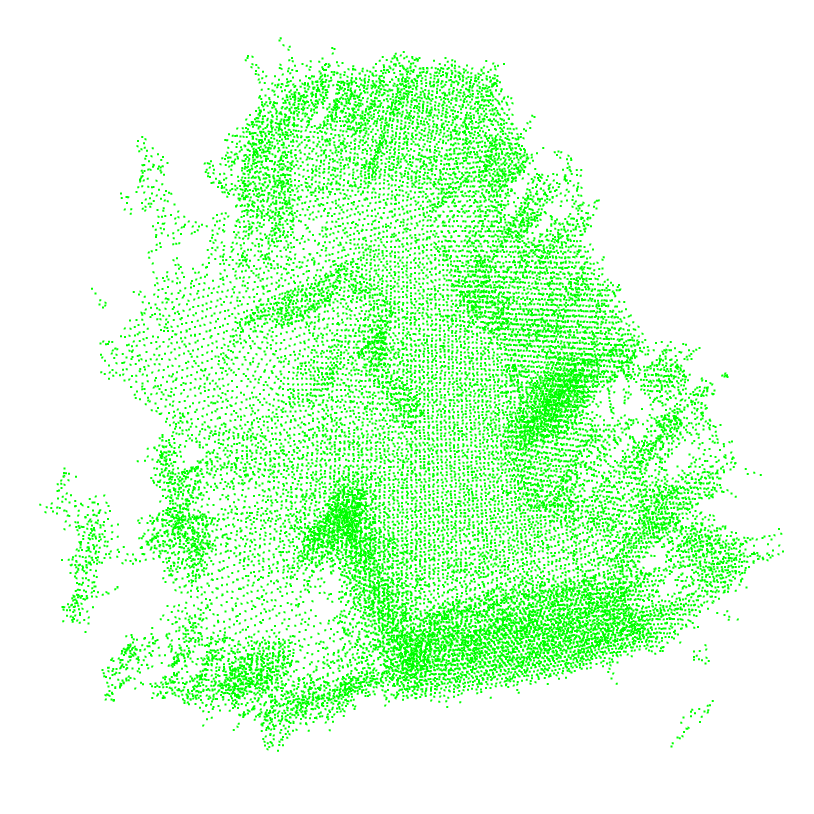
\includegraphics[width=\textwidth]{../img/v1-downsampled.png}
    \caption[Voxelized point cloud map]{Point cloud map voxelized to resolution 0.05 meter per voxel. Notice the regular spacing between points.}
    \label{fig:v1-downsampled}
\end{figure}

Algorithm for voxelization is following. For each voxel (size of the voxel is determined by the resolution) we take all points contained in the voxel and approximate them with their centroid.

As discussed in Section~\ref{chap:analysis}, in a multi-robot system the down-sampling is typically performed by \gls{SLAM} algorithm running on each robot before publishing the map, thus saving bandwidth of the communication. However, in a typical situation, we might want to reduce the resolution even further for the purpose of transformation estimation to reduce the computation time (for example each robot might publish a map with the typical resolution of $0.05$ meters per voxel, but for estimation we work with the resolution of just $0.1$ meters per voxel).

We show in Section~\ref{chap:evaluation} that our algorithm can reliably estimate the transformation for point clouds with $0.1$ meters per voxel resolution.

\subsection{Removing outliers}
\label{sec:outlier-removal}

Although the voxelization can deal with some of the noise and inaccuracies, during experiments it has been beneficial to perform further outliers filtering to remove far laying points. Far-laying outliers may end-up being detected as keypoints, but they are usually not matched. Reducing the number of detected keypoints speeds up the later phases of estimation.

I have selected to use a simple radius-based outlier removal. This method searches for neighbours of each point within a certain radius and removes points that have below threshold neighbours count.

Because descriptors of the outlier points are based on just a few points, which don't produce robust matching candidates, and the radius outlier removal removes only the points with few neighbours, it does not reduce the robustness of the estimation.

For example on two maps from \gls{AAU} dataset (see Section~\ref{sec:aau-dataset}), the outlier removal step removes $326$ and $271$ points respectively ($7.29\%$, $6.16\%$), but the number of detected keypoints decreases from $66, 63$ to $51, 56$ ($22.73\%$, $11.11\%$). Outlier removal didn't impact the estimation process negatively.

\subsection{Estimating surface normals}
\label{sec:normal-estimation}

The last preprocessing step is to estimate surface normals (Figure~\ref{fig:v1-normals}). Surface normals are vectors perpendicular to the surface in the neighbourhood of the point. Surface normals are used in later steps to compute descriptors and by Harris keypoint detector.

\begin{figure}
    \centering
    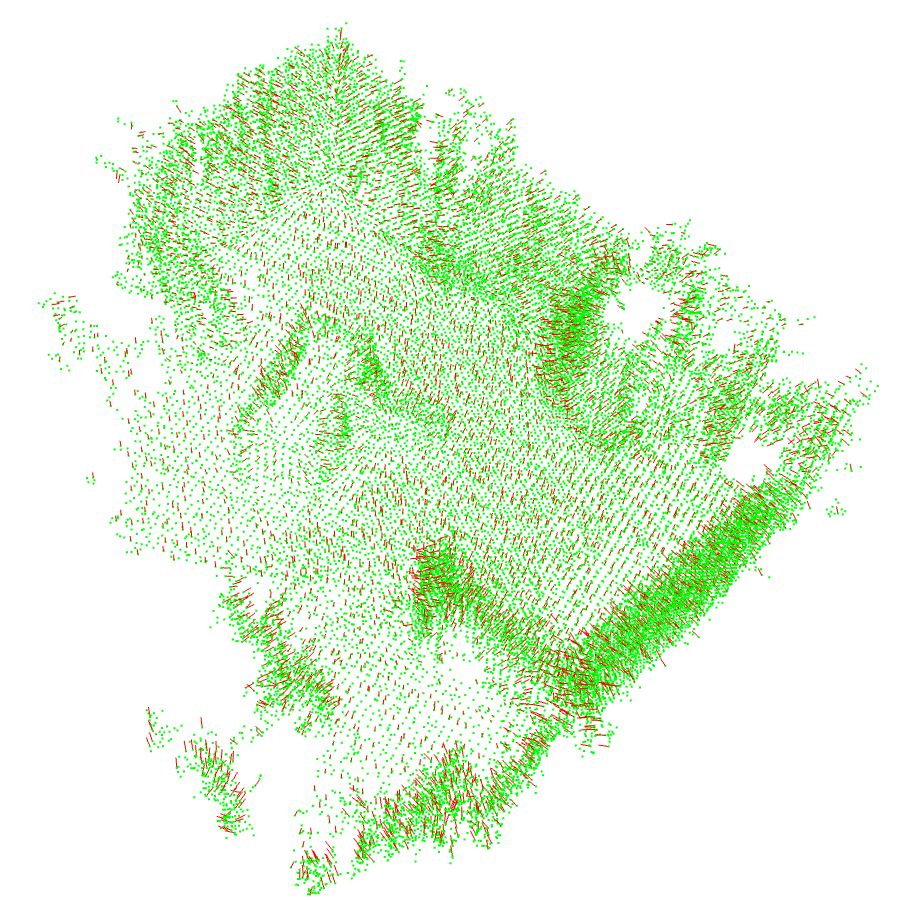
\includegraphics[width=\textwidth]{../img/v1-normals.png}
    \caption[Point cloud map with estimated surface normals]{Voxelized point cloud map with estimated surface normals (red). Only each fifth normal is visualised.}
    \label{fig:v1-normals}
\end{figure}

Algorithm for estimating surface normals is described by~\citet{RusuDoctoralDissertation}. The most important parameter for normals estimation is the size of the neighbourhood which is used for the estimation. This can be configured by the user.

\subsection{Detecting keypoints}
\label{sec:detect-keypoints}

Even after the down-sampling, the maps contain usually too many points to work with all of them in later steps. We need to reduce the number of points further. A common technique used in the area of computer vision and robotics is to search for keypoints that identify suitable points for later matching (Figure~\ref{fig:v1-keypoints}).

\begin{figure}
    \centering
    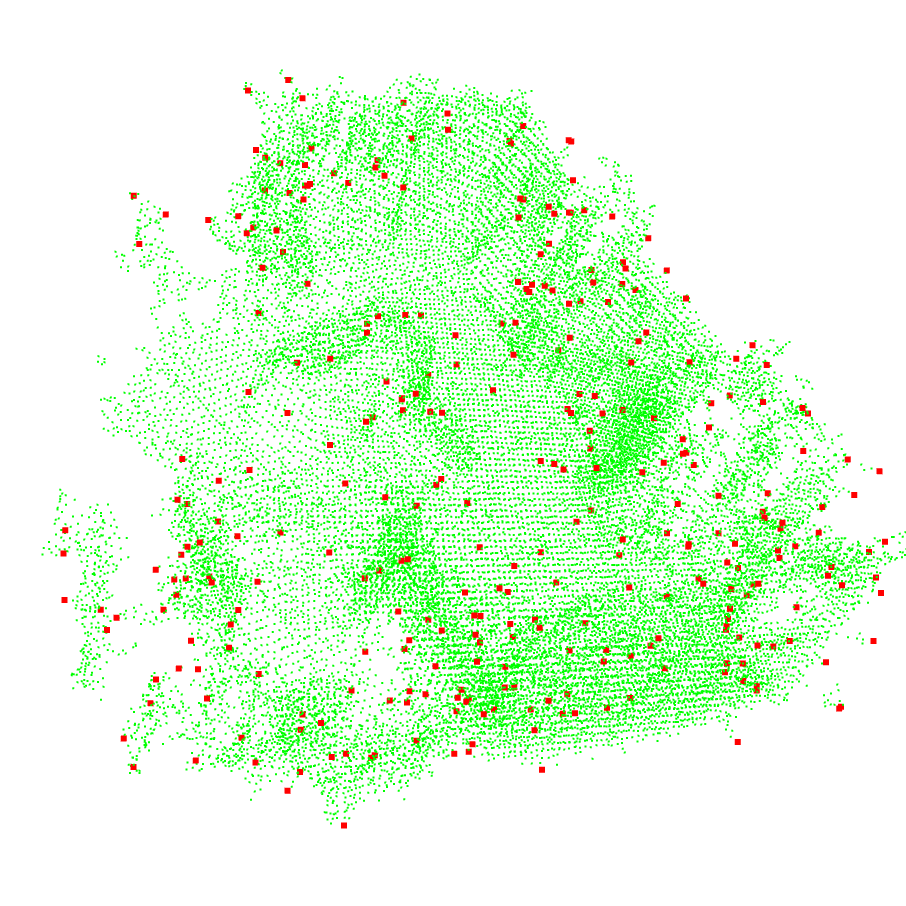
\includegraphics[width=\textwidth]{../img/v1-keypoints.png}
    \caption[Detected keypoints]{\gls{SIFT} keypoints (red) detected in the point cloud map (green).}
    \label{fig:v1-keypoints}
\end{figure}

There are two families of keypoints detectors that are being used with point clouds. Most of the approaches have been adapted from keypoints detectors that have been originally developed to work on images.

The first class of detectors uses \gls{RGB} colour information stored for each point in the point cloud. This approach supposes that the point cloud has been obtained with a detector that provides the colour information such as stereo rig camera setup, active \gls{RGB-D} cameras etc. For the presented approach, I use \gls{SIFT} keypoint detector, which is an adapted algorithm from~\citet{lowe2004distinctive} that works on point clouds with \gls{RGB} information.

The second class of algorithms works with just geometrical information and, therefore, is able to work with point clouds that do not store any additional information for points. These algorithms can be used with point clouds composed of laser scans. Our algorithm implements Harris \gls{3D} keypoint detector for this purpose, which is an adapted algorithm from~\citet{harris1988combined}. Instead of using image gradients, which are not available in the point cloud without colour information, it uses surface normals, that capture geometrical properties of the point neighbourhood.

\subsection{Computing descriptors}
\label{sec:compute-descriptors}

Next step is to compute a local descriptor around each detected keypoint to be able to match keypoints between maps. Unlike the keypoint detection algorithms, algorithms for computing descriptors has been mostly designed from scratch to work on point clouds. A comprehensive review of the descriptors is given by~\citet{YasirThesis}.

Most of the descriptors do not use the colour information and use only local geometry around the point. Widely used \gls{PFH} descriptors, introduced by~\citet{rusu2008pfh}, use a multi-dimensional histogram with $125$ bins to provide an informative signature of a point neighbourhood. The histogram captures relationships between estimated surface normals (see Section~\ref{sec:normal-estimation}). It uses relationships between all pairs of points in the neighbourhood and therefore has complexity $\bigO(k^2)$, where $k$ is the number of points in the neighbourhood. There is a variant of \gls{PFH} descriptors \gls{PFHRGB} that stores also colour information in the extended histogram of $2 \times 125$ bins.

The main disadvantage of the \gls{PFH} descriptors is the high algorithmic complexity and therefore the slow processing speed~\citep{rusu2009fpfh}. Our implementation supports also \gls{FPFH}, introduced by~\citet{rusu2009fpfh}, \gls{SHOT} with colour, introduced by~\citet{tombari2011shot}, \gls{RSD}, introduced by~\citet{marton2010rsd}, and \gls{SC3D}, introduced by~\citet{frome2004sc3d}, novel descriptors which offer better processing speed compared to \gls{PFHRGB} and \gls{PFH}.

\subsection{Matching descriptors}
\label{sec:matching}

Next step in the pipeline is the descriptors matching, which yields an initial transformation estimate. It uses the features extracted from point clouds in the previous steps.

We match two sets of descriptors from two point clouds (Figure~\ref{fig:v1-matching}). For each descriptor from the first set, we want to find a descriptor in the second set, which describes the same place (in the second point cloud). This step is challenging because the descriptors might be less descriptive than desired. Therefore the correct match might not be always the closest descriptor, but the $k$-nearest descriptor.

\begin{figure}
    \centering
    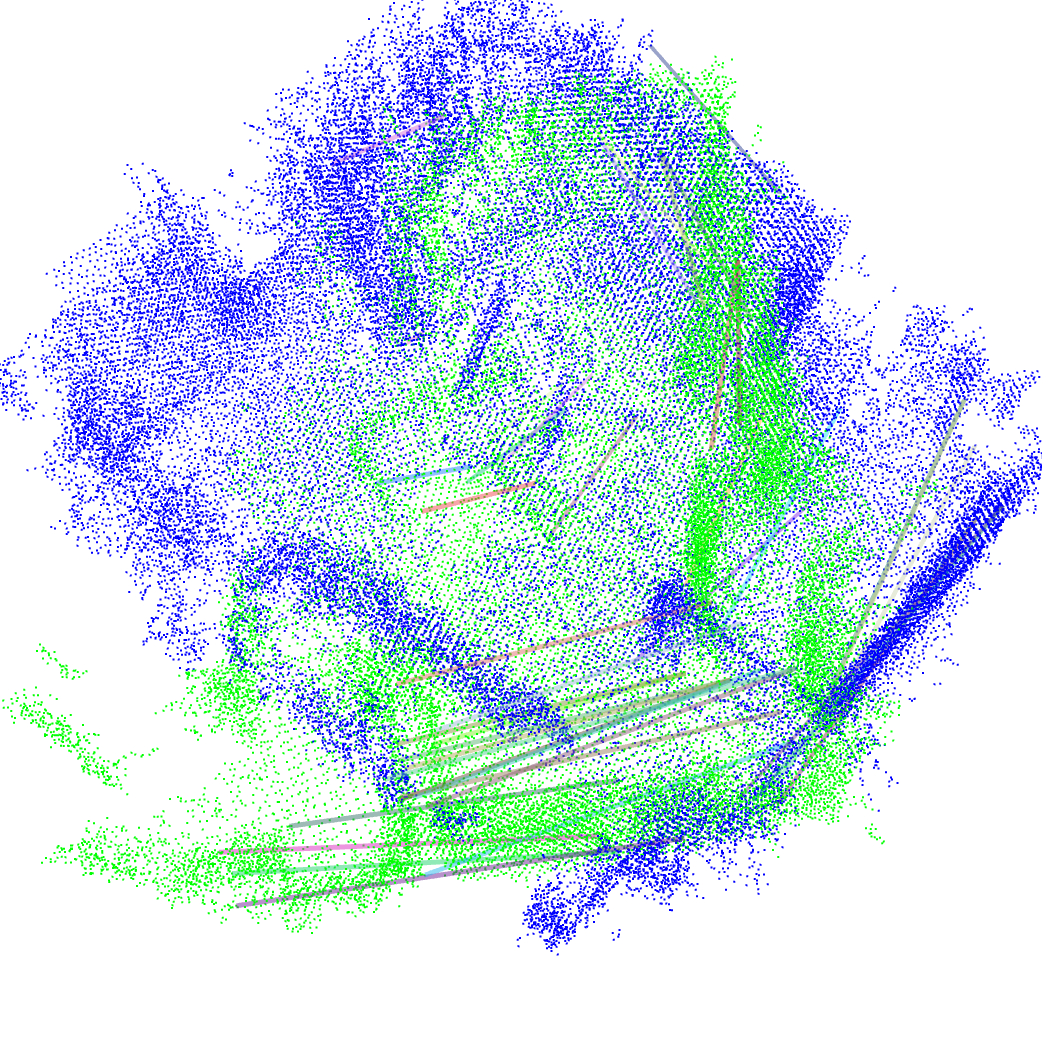
\includegraphics[width=\textwidth]{../img/v1-matching.png}
    \caption[Keypoint matches]{Matched keypoint descriptors between two point cloud maps (green, blue). Only inlier matches from \gls{RANSAC} are shown.}
    \label{fig:v1-matching}
\end{figure}

To overcome the issue, \gls{SAC-IA} algorithm has been proposed by~\citet{rusu2009fpfh} (Algorithm~\ref{alg:sac-ia}).

\begin{algorithm}
    \caption[\gls{SAC-IA}]{\gls{SAC-IA} algorithm from~\citet{rusu2009fpfh}.}
    \label{alg:sac-ia}
    \begin{algorithmic}[1]
        \Require $D_1, D_2$ set of descriptors
        \Ensure rigid transformation estimate
        \Function{\gls{SAC-IA}}{$D_1, D_2$}
            \Loop~repeat $N$ times
                \State $K \gets$ draw $n$ descriptors from $D_1$
                \ForAll{$d_i \in K$}
                    \State $M \gets k$-nearest matches from $D_2$
                    \State $m_i \gets$ a random sample from $M$
                \EndFor
                \State estimate rigid transformation for selected samples
                \State determine inliers
            \EndLoop
            \State \Return transformation with the most inliers.
        \EndFunction
    \end{algorithmic}
\end{algorithm}

The algorithm combines random matching of $k$-nearest descriptors and \gls{RANSAC} algorithm, introduced by~\citet{fischler1981ransac}.

% TODO describe why wanted the new algorithm

The algorithm was originally developed to work with \gls{FPFH} descriptors, that are fast to compute, but less descriptive that \gls{PFH}. With \gls{PFH} and \gls{PFHRGB} descriptors, \gls{SAC-IA} sometimes yields sub-optimal transformation, even when there are good potential matches available in the descriptors sets because it selects matching candidates randomly instead of preferring better matches. This motivated me to develop a new matching algorithm (Algorithm~\ref{alg:cross-match}). This algorithm is deterministic to avoid problems caused by the randomness in \gls{SAC-IA}.

The algorithm is based on the idea of reciprocal match validation. When we are considering match $d_i \rightarrow d_j$, we try to match also $d_j \rightarrow d_i$. We consider all $k$-nearest neighbours for matching to deal with potential low descriptiveness and then select the best match with reciprocal match validation. We do not include \gls{RANSAC} in the scheme, the output of the algorithm is just matched pairs of descriptors.

\begin{algorithm}
    \caption[Reciprocal $k$-nearest matching]{My matching approach using $k$-nearest matches validated with reciprocal matching}
    \label{alg:cross-match}
    \begin{algorithmic}[1]
        \Require $D_1, D_2$ set of descriptors
        \Ensure set of matches between $D_1, D_2$
        \Function{matchReciprocalK}{$D_1, D_2$}
            \State $M = \{\}$
            \ForAll{$d_i \in D_1$}
                \State $N \gets k$-nearest neighbours of $d_i$ in $D_2$
                \ForAll{$d_j \in N$}
                    \State $N' \gets k$-nearest neighbours of $d_j$ in $D_1$
                    \If{$d_i \in N'$}
                        \State $M \gets M \cup \{(d_i, d_j)\}$
                    \EndIf
                \EndFor
            \EndFor
            \State \Return $M$
        \EndFunction
    \end{algorithmic}
\end{algorithm}

Notice that our algorithm does not need any threshold for the maximum match distance and, therefore, can work with various kinds of descriptors without any need for a specific configuration. The only parameter is $k$ -- number of neighbours. As discussed in Section~\ref{chap:evaluation} our approach shows better performance when there are enough good possible matches and is not influenced by randomness.

Both \gls{SAC-IA} and our reciprocal matching algorithm need to quickly find $k$-nearest neighbours. To achieve a good performance we use an approximative nearest neighbour search introduced by~\citet{muja2014flann}. This solution allows us to match a large number of descriptors quickly, even though computational complexity rises significantly with $k$. During the experiments, the matching step takes usually just a fraction of time needed to extract keypoints and descriptors.

\subsection{Estimating the final transformation}
\label{sec:final-estimation}

\gls{SAC-IA} embeds \gls{RANSAC} into its algorithm and therefore provides directly an initial transformation estimate. When we use our matching scheme as per Algorithm~\ref{alg:cross-match}, we need to run \gls{RANSAC} step with rigid transformation model after the matching to get inlier matches. In the typical scenario most of the matches are outliers, so without the \gls{RANSAC} step, it is not possible to estimate a consistent transformation.

\gls{RANSAC} transformation estimate is always based on the minimum number of points required to estimate the model (rigid transformation). To get a better estimate for all inliers pairs we recompute the transformation estimate using least-squares on inlier pairs. We use \gls{SVD} to compute the new estimate, the technique is described by~\citet{golub1970svd}. Another widely used technique in Computer Vision is to use a non-linear least squares approach, such as Levenberg-Marquardt algorithm described by~\citet{more1978levmarq}, to optimize the transformation estimate re-projection error considering all inliers. Because we refine the transformation further with \gls{ICP}, there hasn't been any observed difference between using Levenberg-Marquardt or \gls{SVD}-based technique. The implementation uses \gls{SVD} to refine the transformation on inliers.

So far we have used only detected keypoints and descriptors computed around the keypoints to estimate the transformation. To refine the transformation using all the points in the point cloud we use \gls{ICP} algorithm introduced by~\citet{besl1992icp}. \gls{ICP} algorithm tries to minimize Euclidean error distance between estimated corresponding points (Figure~\ref{fig:v1-refined}). The estimated transformation from either \gls{SAC-IA} or the reciprocal matching scheme presented in Section~\ref{sec:matching} is used as an initial guess for \gls{ICP}.

\begin{figure}
    \centering
    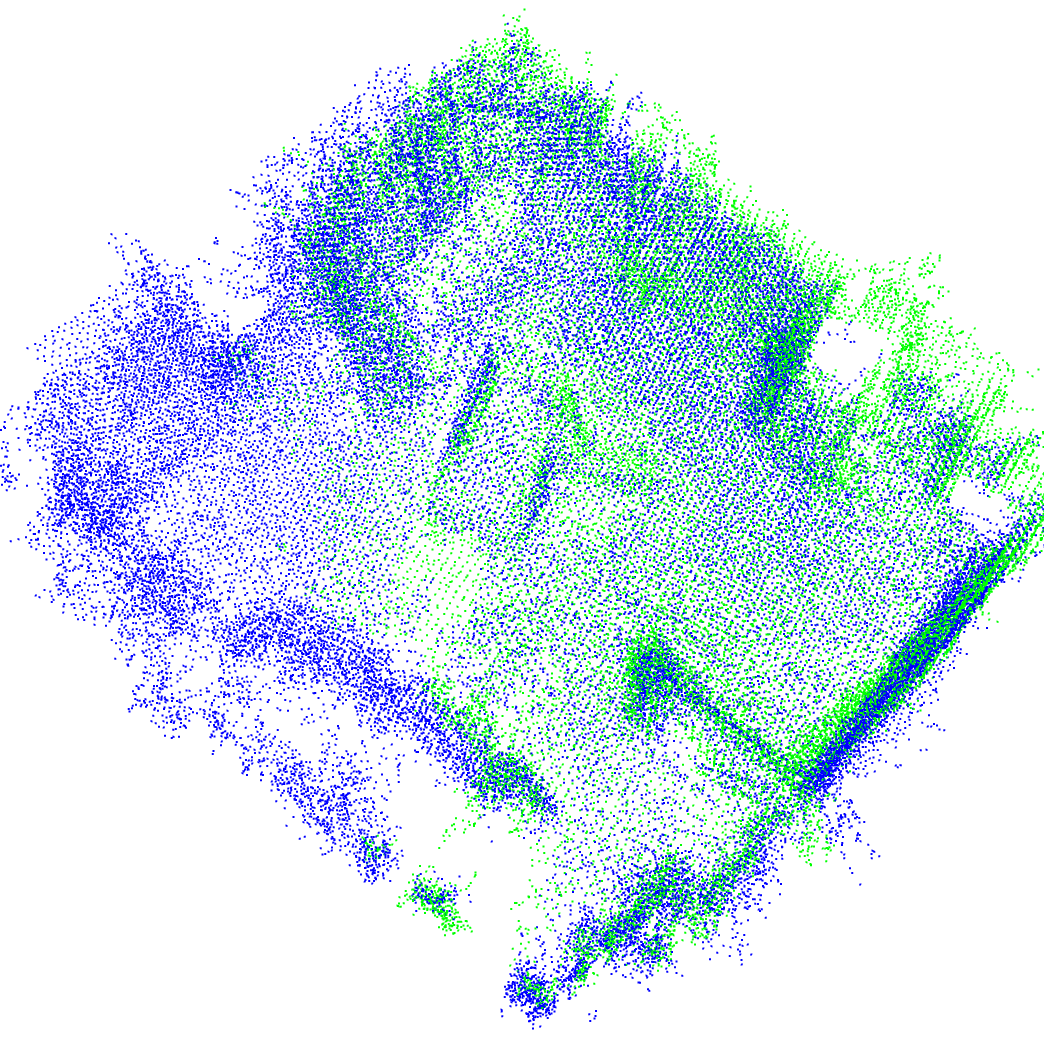
\includegraphics[width=\textwidth]{../img/v1-refined.png}
    \caption[Aligned point clouds]{Two point clouds maps (green, blue) aligned after refining initial transformation with \gls{ICP}. Initial transformation was computed from matches shown in Figure~\ref{fig:v1-matching}.}
    \label{fig:v1-refined}
\end{figure}

The initial guess is usually close to the final transformation estimated by \gls{ICP}, especially when using the reciprocal matching algorithm (Algorithm~\ref{alg:cross-match}) and \gls{RANSAC} for the estimation. Even though we use all the points with \gls{ICP}, because of the proximity of the guess to the final transformation only a couple of iterations is needed for \gls{ICP} to converge, so the refinement does not impact overall performance significantly.

Since the introduction of \gls{ICP}, many \gls{ICP}-derived algorithms have been introduced to overcome issues associated with \gls{ICP}, especially to avoid local minima. A comprehensive review is given by~\citet{pomerleau2015reviewregistration}. Because our initial transformation is usually very close to the final transformation, the original \gls{ICP} algorithm performed well for our use case during experiments.

The \gls{ICP} refinement is the last step in estimating pairwise transformation. We use the output of the \gls{ICP} as the final estimated transformation between two maps.

\subsection{Evaluating the estimated transformation}
\label{sec:transform-evaluation}

To ensure robustness in real-world applications it is valuable to have a confidence measure for the estimated transformation. Commonly used measure for \gls{RANSAC}-based estimates is to use the number of inliers to access the algorithm performance. \citet{brown2007automatic} proposed a probabilistic model for image match verification based on the number of inliers. The authors used model with chosen $\alpha = 8.0$ and $\beta = 0.3$ given by Equation~\eqref{eq:confidence-measure}, where $m$ is the number of matches and $\psi$ is the number of inliers in \gls{RANSAC}.

\begin{equation}
\label{eq:confidence-measure}
\frac{\psi}{8 + 0.3 \cdot m}
\end{equation}

Another possible confidence measure is to use distance error between the two point clouds. This approach is common with point clouds and is implemented in \gls{PCL}. We typically use the Euclidean distance to have a natural metric estimate. This approach has two main issues. Because we do not know the correspondences between two maps we need to use the nearest neighbour for each point to compute the distance. Moreover, to deal with occlusions (points outside intersection of the point clouds) we need to introduce cut-off threshold to deal with too large distances caused by points outside of the intersection.

In the implementation, I use Euclidean distance to evaluate the transformation estimate because the implementation of \gls{SAC-IA} in \gls{PCL} does not provide information about inliers count.

% TODO write algorith for this?

\section{Estimating global transformations}
\label{sec:estimate-global}

The map-merging problem for two maps is discussed in Section~\ref{sec:estimate-pair-wise}. To be able to merge more than two maps we consider a map-merging graph (Definition~\ref{def:map-merging-graph}).

\begin{defn}[Map-merging graph]
    \label{def:map-merging-graph}
    A graph whose nodes correspond to robots' maps and whose edges represent pair-wise transformation estimates between the maps.
\end{defn}

To construct a map-merging graph for $n$ maps we need to estimate $\bigO(n^2)$ pair-wise transformations. Depending on the environment and map relations the map-merging graph might be dense or sparse, but typically will be missing some the edges, because some of the transformations could not be estimated, or could be estimated only with low confidence, see Section~\ref{sec:transform-evaluation}.

Once we have constructed the map-merging graph, the global merged map can be computed by finding a spatial configuration of the nodes (maps) that is consistent with the transformations represented by the edges. In other words, we want to find a transformation for each map from the global reference frame to the particular map consistent with the pairwise transformations.

\subsection{Map-merging as graph-based SLAM}

The idea of a map-merging graph is similar to the idea of a pose graph used in graph-based \gls{SLAM}. Graph-based \gls{SLAM} uses a so-called graph-based formulation of the \gls{SLAM} problem. ``Solving a graph-based \gls{SLAM} problem involves to construct a graph whose nodes represent robot poses or landmarks and in which an edge between two nodes encodes a sensor measurement that constrains the connected poses.''~\citep{grisetti2010tutorial}.

In the graph-based \gls{SLAM} graph, we have poses at different points in time, in the map-merging graph we have maps with origins in unknown positions. In the map-merging graph, we associate our pairwise transformations estimates with edges and in the \gls{SLAM} graph, we use usually direct sensor measurements. In both graphs, we want to find the spatial configuration of the nodes of the graph that is the most consistent with constraints represented by the edges. If we are able to construct the map-merging graph (for which we need to do $\bigO(n^2)$ pair-wise transformation estimates), we can apply the graph-based \gls{SLAM} techniques on the map-merging graph to find the spatial configuration of the nodes that is consistent with our pair-wise estimates. Typically Gauss-Newton, described by~\citet{fletcher2013practical}, or Levenberg-Marquardt algorithm, described by~\citet{more1978levmarq}, are used to optimize the pose graph in graph-based \gls{SLAM}.

To support graph-based \gls{SLAM} approaches, there are libraries specifically focusing on graph optimization under constraints. Well-established examples include \texttt{G2O}, developed by~\citet{kummerle2011g2o}, and \texttt{TORO}, developed by~\citet{grisetti2007toro}. These libraries can be leveraged to solve the map-merging problem for $n$ maps.

\subsection{Solving map-merging problem without loop closures}

Graph optimizing techniques benefit from the presence of loop closures in the graph. During \gls{SLAM} mapping a loop closure occurs when the robot revisits a node in the graph. Loops in the map-merging graph require the robot to be able to estimate pair-wise transformation with at least two neighbours. For example for the shortest loop in the graph, a triangle with three robots, we need each robot to be able to estimate both pair-wise transformations to remaining robots.

Loops in the map-merging graph will usually only occur in fairly large environments and when using many robots. Further on, unlike in graph-based \gls{SLAM}, loop closures may not be critical for good performance of the map-merging algorithm in the typical setup. In the \gls{SLAM} graph, we expect measurements associated with the edges to be subject to the Gaussian noise and corrections based on loop closures are usually vital for good \gls{SLAM} performance. In the map-merging graph, we have pair-wise estimates associated with edges based on the geometry of whole maps containing a large number of points. The pairwise estimates tend to be quite precise because they consider large portions of the environment. There are also available evaluation metrics for the pair-wise estimates (see Section~\ref{sec:transform-evaluation}), which allow us to use only robust estimates in the graph.

Taking advantage of accurate pair-wise estimates in the map-merging graph we may avoid estimating all $\bigO(n^2)$ pair-wise estimates, especially since the pair-wise estimation is the most time-demanding step. To save time we can avoid pair-wise estimates introducing loops in the graph. We can stop pair-wise estimation when the nodes are within one connected component of the graph. We may want to employ a suitable heuristic for selecting the order of pair-wise estimates. Using this approach we might need only $\bigO(n)$ pair-wise estimates to estimate global transformations for the maps.

Below I present fast, non-iterative algorithm (Algorithm~\ref{alg:global-transforms}) for extracting the global poses of maps from the map-merging graph suitable for use in such setup. The algorithm does not take any advantage of the loops in the graph (we expect the use of the approach mentioned above, which avoids loop closures). The algorithm, however, can work with graphs containing loops.

\begin{algorithm}
    \caption[Global poses extraction]{The algorithm to extract global poses of the maps from the map-merging graph (Definition~\ref{def:map-merging-graph}).}
    \label{alg:global-transforms}
    \begin{algorithmic}[1]
        \Require weighted map-merging graph
        \Ensure Transformation for each map from the global reference frame to the map reference frame
        \Function{extractGlobalPoses}{$G = (V, E)$ map-merging graph, $P_e \forall e \in E$ pair-wise transformations estimates}
            \State $C = (V_C, E_C) \gets$ the largest connected component in $G$
            \State $T \gets$ maximum spanning tree of $C$ using confidences as weights
            \State $r \gets$ any node from $T$, selected as the reference frame
            \State $E_s \gets$ edges of $T$ sorted by the distance from $r$
            \State $A_r \gets I$
            \ForAll{$(i,j) \in E_s$}
                \State $A_j \gets A_i P_{(i,j)}$
            \EndFor
            \State $\forall i \not\in V_C: A_i \gets 0$
            \State \Return $A_0, A_1, \dots A_n$
        \EndFunction
    \end{algorithmic}
\end{algorithm}

Because only the maps in the same component of the map-merging graph can be related to the same reference frame, the first step in the algorithm is to extract the largest connected component from the graph. In our setup we expect robots to ultimately form one component and the transformations are computed only for this component. Remaining transformations are set to null transformation. If the robots are expected to operate for a longer period of time separately in multiple components, it might be beneficial for the coordination to compute transformations in all the components, each component having its own reference frame.

Next step in the algorithm is to extract the maximum spanning tree. The edges are weighted with estimated confidence for each pair-wise transformation so that the most confident estimates are used. The possible loops are removed in this step and the non-tree edges are not used.

We can select any node from the spanning tree as the future global reference frame. All the transformations will be computed to this reference frame.

The last step is to compute the transformations to the selected reference frame. For computing the transformation of the node (map) we need transformations on the path from the reference frame (tree root) to the current node to be computed first (actually we need just the preceding transformation, but that implies computing all the transformations). To achieve this we can sort the edges by the distance from the reference node, or just traverse the tree using \gls{BFS} or \gls{DFS} and compute the transformations during the traversal.



\chapter*{Conclusion}
\addcontentsline{toc}{chapter}{Conclusion}

This work presented a novel map-merging algorithm for merging \gls{3D} point cloud maps in multi-robot systems. The algorithm is based on feature-matching transformation estimation and works solely on point cloud maps without any additional auxiliary information. This makes the algorithm applicable in heterogeneous multi-robot systems and the algorithm can work with different \gls{SLAM} approaches and sensor types. To the best of my knowledge the presented approach is the first map-merging algorithm working directly on point clouds without any extra information.

The work showed feasibility of feature-matching approach for registration of low-density point cloud maps produced by \gls{SLAM} algorithms while using \gls{3D} point cloud features typically employed with high-density sensor data.

A reciprocal descriptor matching algorithm was introduced for estimating the initial transformation using feature-matching. The algorithm requires very little parametrisation and exhibited good performance across descriptors in the evaluation. In the most configurations it outperforms \gls{SAC-IA} algorithm for initial alignment available in the \gls{PCL} library.

The map-merging algorithm has been evaluated on real-word datasets captured by both aerial and ground-based robots with variety of stereo rig cameras and active \gls{RGB-D} cameras. It has been evaluated in both indoor and outdoor environments ranging from forest to a single furnished room. The datasets used for evaluation include both well-established benchmark robotics datasets as well as my own experiments.

The proposed algorithm was implemented as a \gls{ROS} package. To the best of my knowledge it is the first \gls{ROS} package for map-merging of \gls{3D} maps. The package has been submitted to the \gls{ROS} distribution, the binary packages are distributed with the \gls{ROS} since the \gls{ROS} Melodic Morenia release. The implementation does not require any particular communication solution between robots and can work with \gls{ROS} in both multi-master and single-master setup. Likewise the implementation does not presume any particular \gls{SLAM} method, nor any particular sensor and uses a portable point cloud map representation, which make it compatible with existing readily available \gls{SLAM} implementations.

While the selected map representation enables great interoperability with existing software, the monolithic point clouds do not permit efficient repairing of mapping errors in the merged map. A pose graph of point clouds representation would be beneficial for the map-merging, but there is no standardised message format in the \gls{ROS} for such a representation nor there is a common graph representation established across different \gls{SLAM} implementations. In the future it would be beneficial to introduce a portable pose graph representation to the \gls{ROS}, as discussed in section~\ref{sec:map-representation}, support it within the core \gls{ROS} packages and promote its usage across \gls{SLAM} implementations. This representation would allow the presented algorithm to work on sub-maps in the pose graph and repair the mapping errors in the merged map.


%%% Bibliography
%%% Bibliography (literature used as a source)
%%%
%%% We employ bibTeX to construct the bibliography. It processes
%%% citations in the text (e.g., the \citet{...} macro) and looks up
%%% relevant entries in the bibliography.bib file.
%%%
%%% The \bibliographystyle command selects, which style will be used
%%% for references from the text. The argument in curly brackets is
%%% the name of the corresponding style file (*.bst). Both styles
%%% mentioned in this template are included in LaTeX distributions.

\bibliographystyle{plainnat}    %% Author (year)
% \bibliographystyle{unsrtnat}     %% [number]

\renewcommand{\bibname}{Bibliography}

%%% Generate the bibliography. Beware that if you cited no works,
%%% the empty list will be omitted completely.

\bibliography{bibliography}

%%% If case you prefer to write the bibliography manually (without bibTeX),
%%% you can use the following. Please follow the ISO 690 standard and
%%% citation conventions of your field of research.

% \begin{thebibliography}{99}
%
% \bibitem{lamport94}
%   {\sc Lamport,} Leslie.
%   \emph{\LaTeX: A Document Preparation System}.
%   2nd edition.
%   Massachusetts: Addison Wesley, 1994.
%   ISBN 0-201-52983-1.
%
% \end{thebibliography}


%%% Figures used in the thesis (consider if this is needed)
\listoffigures

%%% Tables used in the thesis (consider if this is needed)
%%% In mathematical theses, it could be better to move the list of tables to the beginning of the thesis.
% \listoftables

%%% Abbreviations used in the thesis, if any, including their explanation
%%% In mathematical theses, it could be better to move the list of abbreviations to the beginning of the thesis.
% \chapwithtoc{List of Abbreviations}
\printglossary[title=List of Abbreviations,type=\acronymtype]

%%% Attachments to the master thesis, if any. Each attachment must be
%%% referred to at least once from the text of the thesis. Attachments
%%% are numbered.
%%%
%%% The printed version should preferably contain attachments, which can be
%%% read (additional tables and charts, supplementary text, examples of
%%% program output, etc.). The electronic version is more suited for attachments
%%% which will likely be used in an electronic form rather than read (program
%%% source code, data files, interactive charts, etc.). Electronic attachments
%%% should be uploaded to SIS and optionally also included in the thesis on a~CD/DVD.
%%% Allowed file formats are specified in provision of the rector no. 72/2017.
% \appendix
% \chapter{Attachments}

% \section{First Attachment}
\begin{appendices}
\chapter{map\_merge\_3d}
\label{chap:map_merge-wiki}

\end{appendices}

\openright
\end{document}
